\label{ch:corpus}

Nu de structuur en algemene werking van beide systemen is voorgelegd komen de vergelijkende testen. Deze testen zullen op verschillende punten beide systemen evalueren en vergelijken. Volgende punten zijn belangrijk voor systemen die 'Developer Friendly' zijn. Met andere woorden: punten waar ontwikkelaars belang aan hechten bij het kiezen van een framework of CMS voor hun nieuw project \citep{Siddharth200915Framework}.
\newline\newline\noindent
Onderzoeken en staven van volgende punten:
\begin{itemize}
\item Leercurve
\item Documentatie
\item Community
\item Performantie
\item Beheersbaarheid
\item Database structuur
\end{itemize}

\section{Leercurve}
\label{Leercurve}
Elk systeem heeft zo zijn eigen gewoontes en creëert hierdoor een eigen mini-wereld. Zo verschillen systemen in de opbouw van structuur en mappen, naamgevingsconventies, enz. Sommige zijn zeer strikt in gewoontes, andere zeer flexibel. Bij het kiezen van een systeem is het uiteraard belangrijk te kijken naar deze met de minst steile leercurve.

\subsection{Drupal}
Drupal heeft de naam een steile leercurve te hebben. Dit is te nuanceren wanneer we de top van de berg gaan definiëren. Drupal is een relatief eenvoudig systeem om mee van start te gaan. De installatie loopt vlot en na enkele tutorials te volgen moet het mogelijk zijn voor een ontwikkelaar om een eigen thema te creëren, als ook het opstellen van een eenvoudige website. 
\newline\newline
De eerste overwinning om Drupal onder de knie te krijgen is het begrijpen van de verschillende, meestal nieuwe benamingen. Drupal beschikt over een eigen arsenaal van naamgevingsconventies die uniek zijn voor het systeem \citep{Drupal2016CommunityDocumentationb}. Deze lijst bevat een volledig overzicht van alle termen die Drupal gebruikt. Velen hiervan zijn algemene termen die verspreid over de IT-wereld voorkomen. Andere zijn zeer specifiek en nieuw voor de meesten. Termen zoals taxonomy, content type, views, blocks en regions zijn typische specifieke termen.
\newline\newline
Drupal 7 is opgebouwd uit modules. De volgende stap in het leerproces is het begrijpen en configureren van deze modules. De meeste modules spreken voor zich. Toch bestaan er modules die uitgebreide configuratiemogelijkheden hebben. Modules zoals views en rules zijn modules waar configuratie tot in het oneindige loopt. Het beheren en configureren van deze modules vergt enige kennis en ervaring. Kennis kan worden uitgebreid via talloze boeken en tutorials die online te vinden zijn.
\newline\newline
Het bekomen van een resultaat en de weg die gevolgd is, kan steeds op verschillende manieren. Dit is niet anders voor Drupal. Het combineren van verschillende modules tot een werkend en snel geheel kan een uitdaging zijn. Het is geen overbodige luxe op voorhand na te denken welke functies er op de site moeten worden geïmplementeerd en welke module te gebruiker voor welke functie.
\newline\newline
Wanneer we een stuk hoger willen komen op de Drupal berg kan dit inderdaad steil worden. Een ontwikkelaar kent zijn systeem pas echt als hij de werking ervan begrijpt, waarom gebeuren dingen op de manier waarop ze gebeuren? 
\newline\newline
Hoewel er duizenden modules bestaan die een oplossing kunnen bieden voor een bepaald systeem, bestaat de kans dat iets 'custom built' gemaakt moet worden. Hiervoor dien je zelf een module te schrijven of een aftakking van een bestaande module. Het schrijven van een module in Drupal vergt een grondige kennis van de core en werking van het systeem.
\newline\newline
Het creëren van een module ligt buiten de algemene werking voor het opbouwen van een site in Drupal. De ontwikkelaar stapt met andere woorden in een andere wereld. Een volledige oplijsting van een stapsgewijze toer die te volgen is bij het ontwikkelen van een module, is zeer uitgebreid (\cite{Drupal2015ModuleGuide}).

\subsection{OctoberCMS}
In tegenstelling tot Drupal 7 heb je voor het starten aan een eenvoudige website met OctoberCMS wel een basiskennis nodig van HTML, CSS, PHP, SQL en de command-line. Met het bezitten van deze genoemde fundamenten is de leercurve van OctoberCMS eerder klein. 
\newline\newline
OctoberCMS is gebouwd op het PHP framework Laravel. Daarom is het belangrijk de beginselen van Laravel onder de knie te krijgen alvorens van start te gaan met OctoberCMS. Hoewel de folderstructuur en het gebruik van plugins uniek is voor OctoberCMS, is de syntax en werking grotendeels gelijk aan die van Laravel. 
\newline\newline
De opstart van een project met OctoberCMS is zoals eerder aangehaald, snel en eenvoudig. OctoberCMS is modulair opgebouwd en biedt de ontwikkelaar de keuze zijn site op te bouwen via zelf gemaakte plugins, of bestaande plugins terug te vinden op de Marketplace. Met kennis van MVC (Model-View-Controller) is het bouwen van een eigen plugin eenvoudig. Een plugin kan uiteraard veeleisend en erg uitgebreid worden waardoor een grondige kennis van PHP nodig is. Via de Builder plugin wordt het mogelijk om in de back-end van de browser een eenvoudige plugin op te zetten en deze later te configureren in code. 

\subsection{Besluit}
De implementatie van Drupal 7 en OctoberCMS zijn amper te vergelijken. Hoewel ze allebei streven naar hetzelfde resultaat, is de manier waarop geheel anders. Drupal heeft een steile leercurve omdat het algemene werking die een ontwikkelaar normaal hanteert niet aanwezig is bij Drupal 7. Hij kan zijn opgedane kennis in het verleden met andere PHP of Javascript frameworks niet uitspelen in Drupal. Bij OctoberCMS daarentegen kan een ontwikkelaar met kennis van MVC, opgedaan bij andere frameworks, wel aan de slag. De drempel en leercurve voor een ontwikkelaar ligt lager bij OctoberCMS dan bij Drupal 7. 


\section{Documentatie}
De helling van de leercurve van een systeem kan veel te maken hebben met de al dan niet aanwezige documentatie. Bij een systeem met een gebrek aan goede documentatie kan het uitzoeken van een probleem te veel tijd en moeite in beslag nemen. Daarom is het belangrijk alvorens te kiezen voor een bepaald systeem, onderzoek te verrichten daaromtrent. Een goed gedocumenteerd systeem heeft vele voorbeelden, snippet code, artikels en tutorials. Tegenwoordig is het gebruik van screencasts zeer populair. De ideale methode om een leerling visueel en audiovisueel informatie te verschaffen omtrent een onderwerp.

\subsection{Drupal}
Door de jaren heen heeft Drupal een uitgebreide en gestructureerde documentatie kunnen aanleggen \citep{Drupal2016CommunityDocumentation}. Deze documentatie is terug te vinden op de eigenlijke site van Drupal. Maar ook via andere kanalen kan je je kennis verruimen. Het spreekt voor zich dat niet alle bronnen even betrouwbaar zijn, een nuchtere en kritische geest is belangrijk.
\newline\newline

Online leermogelijkheden:
\begin{itemize}
	\item{Drupal.org} \citep{Drupal2016CommunityDocumentation}
	\item{Drupalize} \citep{Drupalize-meDrupalTutorials}
	\item{BuildaModule} \citep{BuildAModule2016BuildAModuleCollections}
	\item{Udemy} \citep{Udemy2016UdemyCourses}
\end{itemize}

\noindent
Gratis alternatieven zijn:
\begin{itemize}
  \item{Youtube}
  \item{Wunderkraut} \citep{FalkJohan2015LearningDrupal}
\end{itemize}

\noindent
Het bijschaven van je kennis kan naast deze online tools ook via tientallen boeken. Let er wel op dat informatie die je verzamelt van vorige versies van Drupal 7 gedeeltelijk of geheel anders kunnen zijn.
\newline\newline

Offline leermogelijkheden: \cite{Drupal2016DrupalMarketplace}
\begin{itemize}
  \item{Programmer's Guide to Drupal, 2nd Edition}
  \item{Pro Drupal as an Enterprise Development Platform}
  \item{The Definitive Guide to Drupal 7}
\end{itemize}

\subsection{OctoberCMS}
In tegenstelling tot Drupal kan OctoberCMS geen beroep doen op jarenlang opgebouwde documentatie. De bèta versie werd gelanceerd op 15 mei 2014. Een officiële release kwam er iets minder dan een jaar later. Op 1 april 2015 werd OctoberCMS als stabiele versie aangeboden \citep{BobkovAlexeyPUTTINGWORDS}.
\newline\newline
Door het korte bestaan van dit systeem kan het toch rekenen op een uitgebreide documentatie met een mooie onderverdeling per segment. Elk pagina bevat bijgevoegde snippet code die de uitleg duidelijk maakt \citep{BobkovAlexey2016OctoberCMSDocumentation}. 

\begin{figure}[!ht]
\begin{subfigure}[b]{0.20\textwidth}
  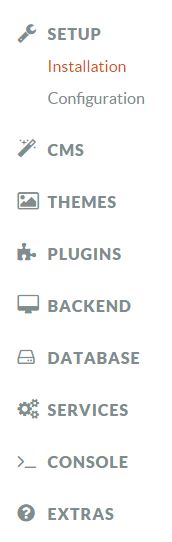
\includegraphics[width=\textwidth]{img/oc-documentation-sidebar.png}
  \centering
  \label{fig:OctoberCMS documentatie over navigatie}
\end{subfigure}
 \hfill
\begin{subfigure}[b]{0.70\textwidth}
 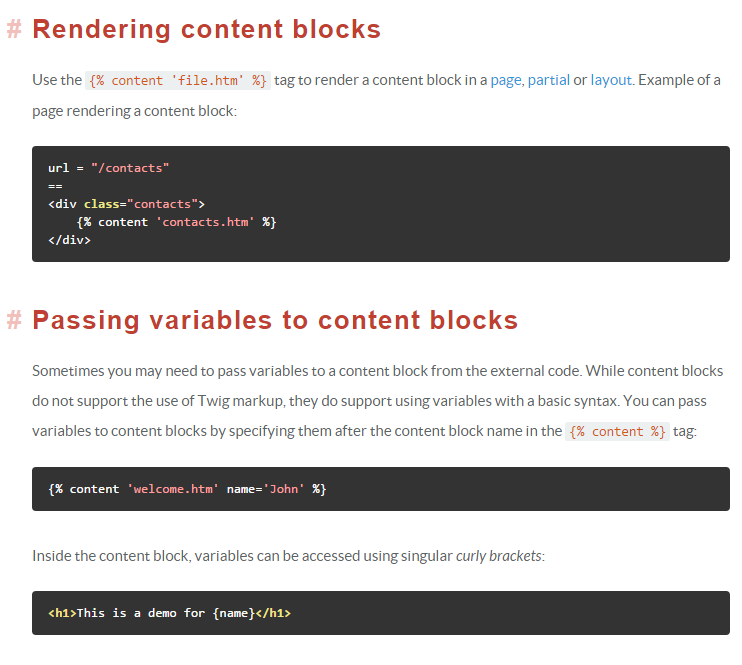
\includegraphics[width=\textwidth]{img/oc-documentation.png}
 \centering
  \label{fig:OctoberCMS documentatie detailpagina}
\end{subfigure}
 
\caption{OctoberCMS biedt een duidelijke documentatie aan op hun officiële site.}
\label{fig:OctoberCMS documentatie}
\end{figure}

\noindent
OctoberCMS beschikt naast documentatie ook over een klein aantal screencasts en tutorials \citep{OctoberCMS2016OctoberCMSRESOURCES} die eerder oppervlakkig zijn en dienst doen als inleiding tot het systeem. Naast de officiële documentatie, screencasts en tutorials die te vinden zijn op de website van OctoberCMS, is er momenteel weinig te vinden. Met uitzondering van twee websites. Sitepoint \citep{SitePoint2016SitePointTutorials}, een verzamelpunt voor ontwikkelaars waarbij ze over verschillende technieken kunnen bijleren aan de hand van tutorials. Sitepoint bevat een bescheiden aantal tutorials die vooral gericht zijn op het ontwikkelen van plugins. De andere site is een blog die de naam Octo-Help \citep{PacurarFilip2015Octo-Help} draagt maar niet rechtstreeks verbonden is met OctoberCMS. Als laatste biedt Youtube nog enkele screencasts aan.

\subsection{Besluit}
Het is duidelijk dat Drupal uitblinkt in de hoeveelheid documentatie en de verschillende kanalen waarop deze te vinden is. Toch kan OctoberCMS als relatief nieuw systeem rekenen op goede documentatie. Al blijft het aantal kanalen nog beperkt. Als built-on systeem van Laravel kan OctoberCMS op vele vlakken rekenen op verdere documentatie van Laravel als terugvalbasis.


\section{Community}
Bij het stoten op een probleem kan een goede community de snelle oplossing bieden. Naast goede documentatie is een goede community cruciaal voor een systeem. Bij het ontwikkelen van een website stoot je gegarandeerd ooit op een probleem dat niet terug te vinden is in documentatie. Dit kan je een heleboel kopzorgen bezorgen wanneer je dit helemaal alleen moet uitzoeken. Bij een goede community kan je via verschillende kanalen je probleem verspreiden. Iedereen kan hierop reageren en helpen mee zoeken naar een oplossing. Indien je probleem reeds voorkwam bij andere personen is de kans groter om sneller een oplossing te vinden. Het toegangsniveau van een community kan ook een belangrijk struikelblok vormen. Bij sommige community's kan de vraagstelling en moeilijkheid hoger liggen dan bij andere. Zo wordt je bijvoorbeeld met een eenvoudige vraag als beginner geconfronteerd met boze blikken en reacties. Krijg je woorden naar het hoofd als RTFM (Read The Fucking Manual). Anderen sturen je door naar de exacte pagina met documentatie. 

\subsection{Drupal}
De Community rond Drupal is onevenaarbaar. Naast een forum waarbij je met alle vragen terecht kan, bestaan er ook Drupal evenementen, sociale media groepen, een Drupal associatie en nog zoveel meer \citep{Drupal2016WhereCommunity}. De kans dat je op nieuw probleem stoot binnen de Drupal wereld is eerder klein te noemen. Zowel via het officiële forum als sites zoals Stack Overflow vind je duizenden posten opgedeeld volgens categorie \citep{Drupal2016CommunityForum}. Via een goede zoekterm of omschrijving van het probleem, kom je ongetwijfeld terecht op een post met hetzelfde probleem en de daarbij horende oplossing(en). Het toegangsniveau van de community is laag. Zowel gebruikers met weinig technische kennis als ervaren ontwikkelaars kunnen er terecht met hun vragen, bedenkingen, ideeën en oplossingen. De onderwerpen gaan van installatieproblemen tot problemen bij het ontwikkelen van modules. 

\subsection{OctoberCMS}
OctoberCMS is niet te vergelijken qua omvang met Drupal. Hoewel dit systeem nog maar een relatief kort bestaan heeft is de community er rond sterk gegroeid de afgelopen maanden. Oorspronkelijk werd dit systeem door twee personen opgebouwd. Nu zijn er maar liefst 141 personen die deelnemen aan het verbeteren van de core van OctoberCMS \citep{OctoberCMS2016OctoberCMSGithub} en 38 personen die de documentatie verder aanvullen en verbeteren \citep{OctoberCMS2016OctoberCMSDocumentation} (Geraadpleegd op 14-05-2016).
\newline\newline
Het support forum van OctoberCMS bevat verschillende onderverdelingen. Gaande van 'Best Practices', help en ondersteuning, tot nieuws en aankondigingen. De support bevat een kleine 1500 posten die al dan niet een antwoord bieden op de gestelde vraag. Vragen kunnen onbeantwoord blijven omdat er momenteel nog geen eenduidige oplossing voor gevonden is. De support op andere sites zoals Stack Overflow blijven beperkt. De Live Chat biedt een snelle respons voor specifieke vragen. 

\subsection{Besluit}
Zoals reeds aangehaald is de Community rond Drupal onevenaarbaar. De oplossing voor vragen en problemen zijn ongetwijfeld te vinden op het internet. Alleen kan het moeilijk worden de juiste oplossing binnen een aanvaardbare tijdspanne te vinden. Het aantal posten omtrent sommige onderwerpen kunnen oplopen in de honderden. Het ingeven van specifieke zoektermen is de boodschap. OctoberCMS daarentegen komt op dit vlak soms te kort. Ik haalde reeds aan dat het aantal posten beperkt blijft tot 1500 stuks., al dan niet beantwoord. Dit is aan de lage kant aangezien dit een verzameling is van allerhande soorten onderwerpen. Dit is te verklaren door het eerder korte bestaan en het beperkt aantal gebruikers van OctoberCMS. Het vinden van een oplossing voor een probleem bij OctoberCMS kan ook buiten de aanvaardbare tijdspanne vallen waardoor dit een gebrek kan zijn voor bijhorende oplossingen voor gelijkaardige problemen.


\section{Performantie}
Performantie is een vanzelfsprekend belangrijk element bij het kiezen van een systeem. Hoe snel wordt een pagina opgehaald en visueel voorgesteld aan de eindgebruiker, wat en hoe verbetert een systeem zijn performantie. Dit zijn factoren die belangrijk zijn voor de ontwikkelaar maar zeker ook voor de eindgebruiker/klant.
\newline\newline
Drupal en OctoberCMS werden beide getest op performantie. Deze testen werden lokaal uitgevoerd waarbij beide systemen dezelfde functies (pagina's) hebben. De performantie testen zijn uitgevoerd via de ontwikkel extensie in Google Chrome. Via deze extensie is het onder andere mogelijk HTML en CSS elementen te inspecteren, bronbestanden op te vragen en netwerkgegevens op te halen. Via de tab netwerkgegevens kan je de performantie van elke pagina onder de loep nemen. Nagaan welke bestanden worden ingeladen en hoelang het effectief duurt vooraleer de volledige pagina ingeladen is. Er kan gesimuleerd worden voor verschillende netwerksnelheden en types. De homepagina zal onderworpen en geëvalueerd worden aan performantie prestaties. Naast de front-end bekijken we of de laadtijd verschillend is met de back-end. We onderwerpen een content pagina aan de performantie test.

\subsection{Drupal}
Drupal is nooit de beste performer geweest uit het pak. Het willen voldoen aan ieders noden om een zo wijd mogelijk toepassingsgebied te creëren resulteert in een te zware en grote 'codebase' of basiscode. Een project gebruikt nooit de volledige capaciteit van wat het systeem aankan maar bevat wel de overbodige functionaliteiten die niet gebruikt worden. Deze ongebruikte functionaliteiten vertragen derhalve. De architectuur van het systeem om deze ongebruikte functionaliteiten te gaan aanspreken zullen ook een impact geven op de performantie. 
\newline\newline
De manier waarop Drupal hiermee omgaat om de performantie op te drijven is via caching. Drupal cached overal waar het kan. Gaande van de database query resultaten, de front-end resources, enz. Dit is op zich geen probleem bij sites waar enkel en alleen content getoond moet worden door anonieme gebruikers. Wanneer de site intensief gebruikt wordt door geautoriseerde personen die content inladen en aanpassen, biedt caching niet de ideale oplossing.
\newline\newline
We onderwerpen de homepagina aan een performantie test. We zien dat een eerste lading van de pagina, volledig geladen (Load) is op 1.23 seconden. De laadtijd voor de initiële opmaak (DOMContentLoaded) bedraagt slechts 854 milliseconden. De totale grootte die ingeladen moet worden voor de index pagina is 1.5MB. Via het overzicht kunnen alle files gedetailleerd bestudeerd worden.

\begin{figure}[!ht]
  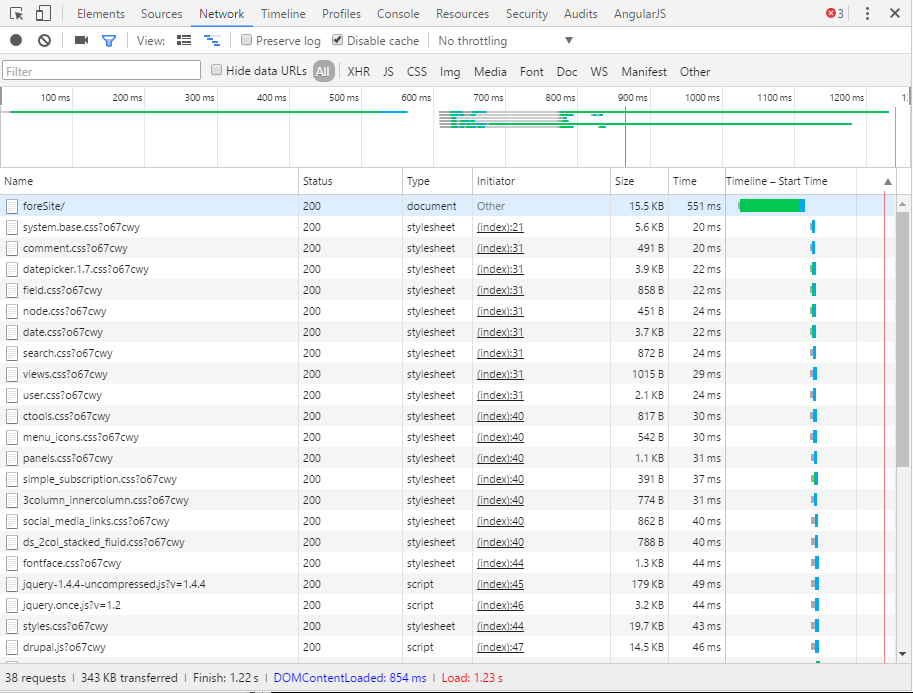
\includegraphics[width=\textwidth]{img/dr-performance-test.png}
  \caption{Drupal performantie test: overzicht van het resultaat.}
  \label{fig:Drupal performantie test.}
\end{figure}

\pagebreak

\begin{table}[!ht]
\centering
\begin{tabular}{|l|c|r|}
    \hline
    Laden pagina & Laadtijd opmaak & Laadtijd volledige pagina\\
    \hline
    1ste & 0.854s & 1.23s\\
    \hline
    2de & 0.905s & 1,44s\\
    \hline
    3de & 0.844s & 1.23s\\
    \hline
    4de & 0.842s & 1.36s\\
    \hline
    5de & 0.819s & 1.19s\\
     \hline
    6de & 0.842s & 1.22s\\
    \hline
    Gemiddelde & 0.851s & 1.28s\\
    \hline
\end{tabular}
\caption{\label{tab:Drupal resultaten performantie front-end } Een overzicht van de laadtijden van de index pagina.}
\end{table}

\noindent
De index pagina wordt geladen met een gemiddelde snelheid van 1.28 seconden. Dit is op zich behoorlijk veel als we dit vergelijken met sommige andere frameworks die een laadtijd hebben van 20 tot 100ms. We bekijken of de front-end laadtijd verschillend is met de back-end laadtijd.

\pagebreak

\begin{table}[!ht]
\centering
\begin{tabular}{|l|c|r|}
    \hline
    Laden pagina & Laadtijd opmaak & Laadtijd volledige pagina\\
    \hline
    1ste & 0.897 & 3.00s\\
    \hline
    2de & 1.67s & 3.82s\\
    \hline
    3de & 1.10s & 2.93s\\
    \hline
    4de & 0.891s & 2.95s\\
    \hline
    5de & 1.43s & 3.11s\\
     \hline
    6de & 1.05s & 4.35s\\
    \hline
    Gemiddelde & 1.188s & 3.36s\\
    \hline
\end{tabular}
\caption{\label{tab:Drupal resultaten performantie back-end } Een overzicht van de laadtijden van de back-end pagina.}
\end{table}

\noindent
Het wordt duidelijk dat de laadtijden van de front-end een stuk lager liggen dan deze aan de back-end zijde. Het verschil tussen de laadtijd van de initiële opmaak en de volledige laadtijd is immens. De back-end van Drupal wordt bovenop de front-end afgebeeld als een soort van laag. Dit verklaart het verschil tussen de laadtijd van de initiële opmaak en de volledige pagina. De laadtijd van de initiële opmaak is de tijd die nodig is om de front-end af te beelden. De overige tijd is nodig om de back-end in de laden bovenop de front-end pagina. 

\begin{figure}[!ht]
  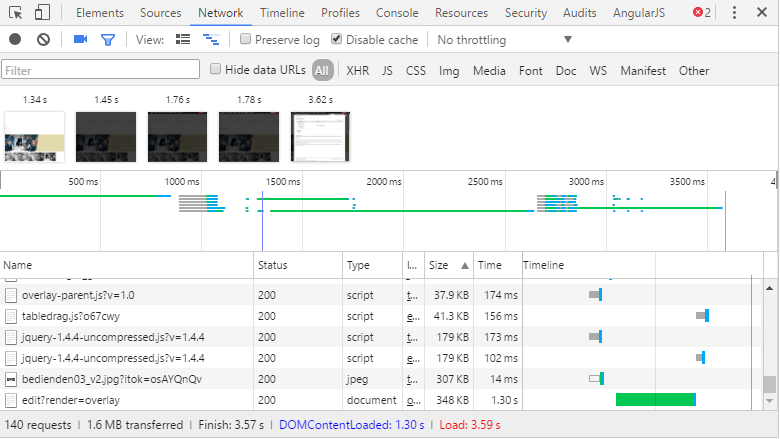
\includegraphics[width=\textwidth]{img/dr-performance-test-backend.png}
  \caption{Drupal performantie test: overzicht van het resultaat van de back-end pagina.}
  \label{fig:Drupal performantie test back-end.}
\end{figure}

\pagebreak


\subsection{OctoberCMS}
OctoberCMS is zeker geen uitschieter als het over performance gaat. Nochtans is de structuur en files volledig beheersbaar. Aangezien OctoberCMS bovenop Laravel draait en dit systeem een grote codebase heeft, vertraagt dit het volledige systeem. Standaard wordt slechts weinig in de cache opgeslagen, dit kan manueel beheerd worden waardoor performance prestaties kunnen verbeterd worden.
\newline\newline
Wanneer we de homepagina van OctoberCMS onderwerpen aan performantie prestaties kunnen we zien dat de laadtijd van de volledige pagina (Load) 1.88 seconden bedraagt. Het verschil tussen laadtijd van de volledige pagina en de initiële opmaak (DOMContentLoaded) is te verwaarlozen. De homepagina heeft een grootte van 576KB die verdeeld wordt over 15 bestanden. Via het overzicht kan voor elk bestand de grootte, laadtijd en volgorde van uitvoering, uitvoerig bestudeerd worden.

\begin{table}[!ht]
\centering
\begin{tabular}{|l|c|r|}
    \hline
    Laden pagina & Laadtijd opmaak & Laadtijd volledige pagina\\
    \hline
    1ste & 1.88s & 1.90s\\
    \hline
    2de & 2.02s & 2.02s\\
    \hline
    3de & 2.08s & 2.11s\\
    \hline
    4de & 1.94s & 1.96s\\
    \hline
    5de & 1.88s & 1.89s\\
     \hline
    6de & 2.02s & 2.05s\\
    \hline
    Gemiddelde & 1.97s & 1.98s\\
    \hline
\end{tabular}
\caption{\label{tab:OctoberCMS resultaten performantie front-end } Een overzicht van de laadtijden van de index pagina.}
\end{table}

\noindent
De index pagina wordt ingeladen met een gemiddelde snelheid van 1.98 seconden. Dit is eerder aan de trage kant. We vergelijken de laadtijden van de front-end nu met deze van de back-end.

\begin{table}[!ht]
\centering
\begin{tabular}{|l|c|r|}
    \hline
    Laden pagina & Laadtijd opmaak & Laadtijd volledige pagina\\
    \hline
    1ste & 2.31s & 2.39s\\
    \hline
    2de & 2.96s & 3.03s\\
    \hline
    3de & 2.39s & 2.43s\\
    \hline
    4de & 2.27s & 2.30s\\
    \hline
    5de & 2.36s & 2.40s\\
     \hline
    6de & 2.37s & 2.42s\\
    \hline
    Gemiddelde & 2.44s & 2.49s\\
    \hline
\end{tabular}
\caption{\label{tab:OctoberCMS resultaten performantie back-end } Een overzicht van de laadtijden van de back-end pagina's.}
\end{table}

\noindent
De gemiddelde laadtijden voor de back-end pagina's liggen ongeveer een halve second hoger. Hoewel dit op het eerste zicht weinig lijkt, kan dit beduidend trager aanvoelen voor de gebruiker.

\begin{figure}[!ht]
  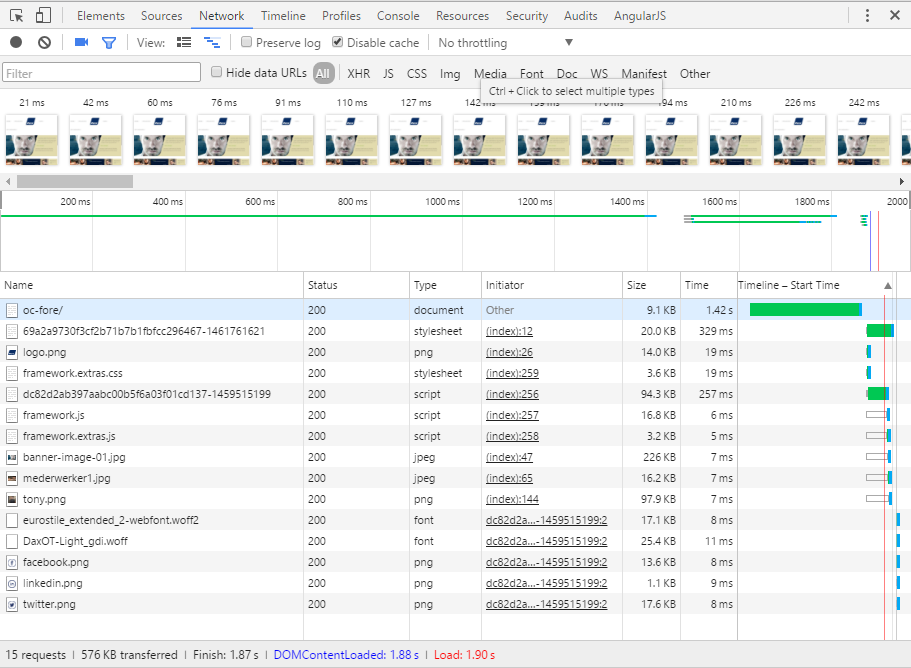
\includegraphics[width=\textwidth]{img/oc-performance-test.png}
  \caption{OctoberCMS performantie test: overzicht van het resultaat.}
  \label{fig:OctoberCMS performantie test.}
\end{figure}


\subsection{Besluit}
We kunnen vaststellen dat beide systemen niet de beste laadtijden neerzetten. De verschillen tussen het laden van de front-end en de back-end pagina's zijn bij Drupal groot. Bij OctoberCMS is er ook een duidelijk verschil maar dat is niets in vergelijking met Drupal.
\newline\newline
Mits een goede caching kan de laadtijd van OctoberCMS een stuk verminderd worden. Maar een laadtijd neerzetten onder de 100 milliseconden, zoals heel snelle systemen, zit er niet in.


\section{Beheersbaarheid}
De beheersbaarheid van een systeem is de mate waarin een systeem 'Developer Oriented' is. In welke mate is het systeem ontworpen voor ontwikkelaars. Veelal worden CMS systemen met oog op de eindgebruiker gemaakt. Dit zijn mensen zonder enige of geringe technische kennis omtrent programmeren. Deze systemen zijn ontworpen om de mogelijkheid te scheppen voor deze mensen om een eigen basis site op te stellen. Ontwikkelaars kunnen hiermee ook aan de slag om verder te gaan dan een basis site. Beheersbaarheid staat gelijk aan de controle die er al dan niet is in verband met coding, theming, foutboodschappen, enz.

\subsection{Drupal}
Drupal is ontworpen met de intentie om minder technische mensen ook de kans te geven een eenvoudige website op te bouwen via hun systeem. Ontwikkelen via Drupal is niet altijd een plezier. Ontwikkelen van een basissite in Drupal is niet moeilijk te noemen qua programmering, maar het kan veel moeite kosten het concept en de flow ervan onder de knie te krijgen. Het is ook niet altijd duidelijk welke aanpassingen welke gevolg hebben.
\newline\newline
Belangrijk bij het starten van een project met Drupal is vooraf het project 100 procent te definiëren, zodat de structuur kan vastgelegd worden. Veranderlijke projecten waarbij elementen doorheen de implementatie veranderen zijn geen opdracht voor Drupal.
\newline\newline
\subsubsection{Coding}
Coding, of de manier waarop code geschreven en beheerd wordt in een systeem. Bij Drupal 7 is het mogelijk een volledige site op te stellen zonder ook maar één regel code te schrijven. Alles verloopt hier via de back-end van de browser. Zoals eerder aangehaald kan de structuur van verschillende pagina's en nodes worden aangepast door template bestanden te overschrijven van de core bestanden. Qua beheersbaarheid is dit niet ideaal. Elke module kan één of meerdere template bestanden bevatten die elk apart overschreven moeten worden. Natuurlijk is het niet verplicht alle template bestanden te gaan overschrijven. Toch is het aan te raden zeker de page.tpl.php te overschrijven om de structuur van je 'body' aan te passen.
\newline\newline
Een andere reden om de template bestanden te overschrijven is om propere code te verkrijgen. Drupal 7 levert default niet bepaald propere code af. Een teveel aan div-tags die te diep genest zitten, meestal zonder enige meerwaarde aan je code. Daarnaast voegt Drupal 7 een heel arsenaal klassen toe aan deze div-tags. Klassen die veelal weinig concrete info verstrekken over de inhoud van de sectie. Het stijlen van deze klassen en daarbij het overzicht bewaren, is een hele opdracht. In de meeste gevallen is het wel mogelijk om manueel een klassennaam toe te voegen aan het gewenste element. Er is een mogelijkheid om aan ieder veld van een content type een unieke klasse toe te voegen. Dit verandert uiteraard niets aan het uitzicht van de code, maar geeft wel een mogelijkheid om dit item uniek te gaan stijlen. 

\begin{figure}[!ht]
  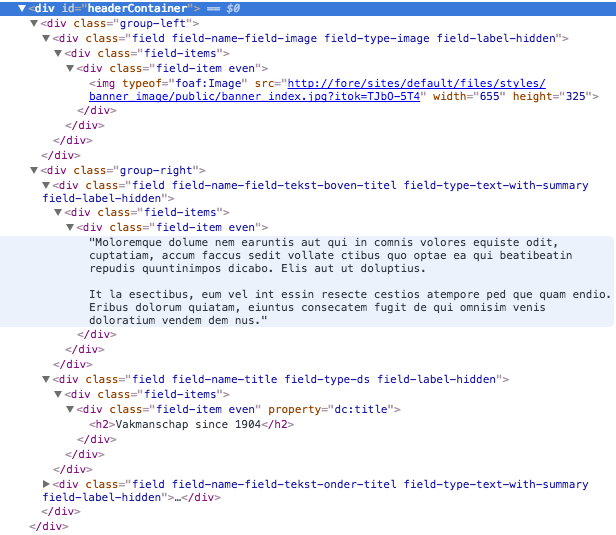
\includegraphics[width=\textwidth]{img/dr-htmldiv.png}
  \caption{Drupal's HTML code om de Header te tonen is allesbehalve proper en overzichtelijk te noemen.}
  \label{fig:Drupal html structuur.}
\end{figure}

\noindent
Via het overschrijven van template files kunnen een teveel aan div-tags verwijderd worden om zo de code minimaal op te poetsen. De overbodige en weinig omschrijvende klassen kunnen vervangen of verwijdert worden door concrete, eigen gekozen namen.
\newline\newline
Inhoud kan enkel worden aangemaakt en gecontroleerd via de back-end van de browser. Dit kan beperkingen opleveren. Er is te weinig controle over de structuur die de inhoud aanneemt. Deze controle kan gedeeltelijk opgevangen worden door modules die inhoud kunnen groeperen, filteren en herschrijven. De module display suite geeft de mogelijkheid velden te groeperen en ordenen. De views module zorgt ervoor dat er gefilterd kan worden en dat velden herschreven kunnen worden. Hoewel dit in de meeste gevallen een oplossing kan bieden, blijft dit een omslachtige manier van werken en is alles behalve gunstig als ontwikkelaar. In het andere geval is het zoeken naar een module die hopelijk een oplossing kan bieden.
\newline\newline
Een ander nadeel van het database georiënteerde systeem is het gebrek aan duplicatie van code. Aangezien bijna alles via de database verloopt is het moeilijk om een bepaalde actie of configuratie op net dezelfde manier uit te voeren. Een configuratie die in de ene site naar behoren werd afgeleverd kan niet eenvoudigweg gekopieerd worden naar een ander project die een gelijkaardige configuratie vraagt.

\subsubsection{Foutboodschappen}
Foutboodschappen tijdens het programmeren kunnen een cruciale bron van informatie zijn. Zonder concrete aanwijzing van het probleem kan dit uitdijen in een zoektocht. Drupal beschikt over drie opties als het op foutboodschappen aan komt. Wanneer je site in productiemode draait kies je best om geen foutboodschappen weer te geven. Dit komt allesbehalve goed over naar de eindgebruiker. In ontwikkelmodus kan je kiezen om alle berichten weer te geven of enkel fouten en gevaren. 
\newline\newline
Over het algemeen wordt je amper slimmer bij het bekijken van foutboodschappen in Drupal. Veelal zullen deze database gericht zijn, aangezien zowat alle acties die uitgevoerd worden connectie met de database vragen. Foutboodschappen worden op het eerste zicht gedetailleerd getoond met een beschrijving, lijnnummer en bestandsreferentie. Als we kijken waar deze file zich bevindt, merken we op dat dit uit een module komt. Een geïnstalleerde module die simpelweg geïnstalleerd is en waar verder geen aanpassingen aan gedaan zijn. Even de cache legen kan hopelijk het probleem oplossen. Anders kan je met deze info hooguit aan de slag door deze foutboodschap in te geven als zoekterm in Google.
 
\pagebreak

\begin{figure}[!ht]
  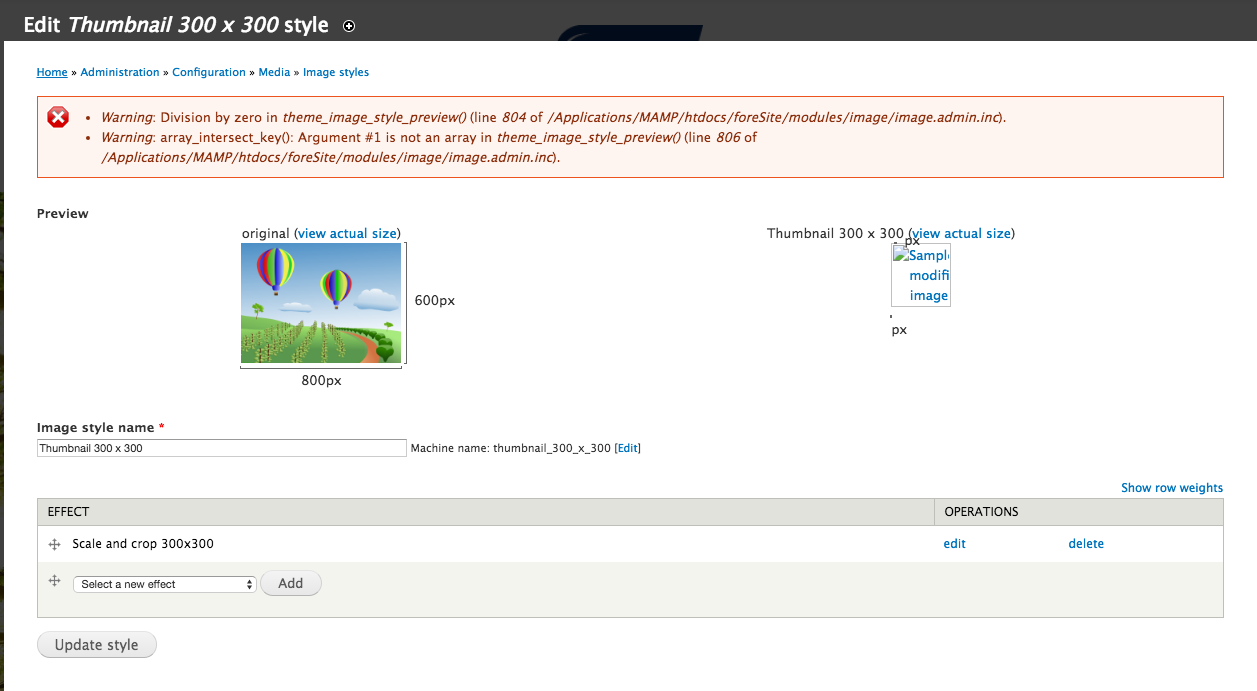
\includegraphics[width=\textwidth]{img/dr-errors.png}
  \caption{Een foutboodschap in Drupal die weinig beschrijvende info bevat.}
  \label{fig:Drupal foutboodschap.}
\end{figure}

\noindent
Een ander frustrerend fenomeen binnen Drupal is het WSOD (white screen of death). Het kan gebeuren dat je als gebruiker stoot op een volledig witte pagina. Deze pagina bevat geen inhoud, foutboodschappen of waarschuwingen. De oorzaak van dit probleem kan vele redenen hebben. Indien je site in productie staat kan het zijn dat fouten uitgeschakeld zijn waardoor de foutboodschap niet zichtbaar is. Wanneer dit niet het geval is en er nog steeds niets verschijnt, kan de foutboodschap(pen) geforceerd getoond worden door het index.php bestand aan te passen. Voeg net na de opening van de PHP tag volgende code toe.

\begin{minted}{c}
  error_reporting(E_ALL);
  ini_set('display_errors', TRUE);
  ini_set('display_startup_errors', TRUE);
\end{minted}

\noindent
Dit zal alle mogelijke foutboodschappen op het scherm tonen. Enkel geheugenfouten zullen niet zichtbaar zijn. 


\subsubsection{Versiebeheersysteem}
In de meeste gevallen worden IT-projecten zelden ontwikkeld door slechts één persoon. Zo zullen bij het ontwikkelen van websites de taken meestal verdeeld worden tussen front-end en back-end: twee of meerdere personen die een stuk van de opbouw van een website voor hun rekening nemen. De beste manier om samen te werken in groep aan één of meerdere projecten is door gebruik te maken van een versiebeheersysteem. Code wordt extern op een server bewaard waar desbetreffende personen toegang tot hebben. Het meest bekende versiebeheersysteem is zonder twijfel Git.
\newline\newline
Versiebeheersystemen kunnen verschillende doeleinden hebben. Gaande van kleine statische of dynamische websites tot grotere applicaties. 
\newline\newline
Een versiebeheersysteem maakt gebruikt van een bestandsgebaseerde opslagmethode. Drupal slaat de meest belangrijke data op in een relationele database, waardoor versiebeheer een stuk moeilijker wordt. Alle inhoud en configuratie van deze inhoud (content types), views, menu's en nog zoveel andere informatie, worden via de browser ingegeven en opgeslagen in de database. Bij een versiebeheer met een bestandsgebaseerde opslagmethode kan er bij een fout eenvoudig worden teruggegrepen naar vorige code. Aanpassingen doorgevoerd in Drupal zijn permanent doorgegeven aan de database. 
\newline\newline
Het is uiteraard mogelijk om te werken met een versiebeheersysteem, alleen wordt de kans op conflicten in de database een stuk groter en is de werking behoorlijk omslachtig. Exporteer de database en sla deze op in de map projectnaam > sites > default. Nu kan deze worden gepusht naar de externe server. Importeren werkt op dezelfde manier. Deze manier van werken kan problemen geven wanneer twee of meer personen op dezelfde moment aanpassingen doen en op deze manier de database gaan beïnvloeden. Aangezien bijna alle taken via de database verlopen, is de kans groot dat dit zal voorkomen. Deze methode kan werken wanneer de ene persoon zich enkel bezighoudt met het stijlen van de website via code in CSS, en de andere, andere structurele taken uitvoert die de database beïnvloeden.


\subsection{OctoberCMS}
OctoberCMS werd volledig met het oog op ontwikkelaars gemaakt. Het systeem is volledig bestandsgebaseerd en biedt daardoor een volledige controle aan de ontwikkelaar. De back-end in de browser wordt getoond in een mooi en duidelijk design. Het gebruik ervan is intuïtief en bevat geen overdrive aan elementen.

\subsubsection{Coding}
Alle code die geschreven is, is aanpasbaar naar eigen wens. De controle over HTML, CSS, Javascript ligt volledig in de handen van de ontwikkelaar. Het gebruik van partials en layout pagina's bevordert de herbruikbaarheid van code en behoudt het overzicht bij grote projecten. Content blocks kunnen beheerd worden door de eindgebruiker alsook de ontwikkelaar. Aanpassingen kunnen in code of in de back-end van de browser via een WYSIWYG. Dit is een teksteditor waarbij de eindgebruiker de opgemaakte tekst direct ziet en de kans heeft deze aan te passen.
\newline\newline
Toevoegen van bestaande plugins kan simpelweg via de back-end in de browser. Eenmaal geïnstalleerd kunnen componenten gesleept worden in de editor en wordt er automatisch snippet code aangemaakt. Dit is de meest eenvoudige manier van werken. Voor geavanceerd gebruik kan de code ook worden getoond en aangepast waar nodig. Het aanmaken van nieuwe plugins kan op verschillende manieren (eerder besproken) en hoeft niet moeilijk te zijn. Een plugin kan uiterst geavanceerd worden afhankelijk van de functies waaraan hij moet voldoen.
\newline\newline
Het aanmaken van een nieuw thema is centraal beheerd. Alle mappen en bestanden die behoren tot het thema, bevinden zich in diezelfde map. Geen gedoe met uitzoeken waar welke stukken code worden aangemaakt en beheerd. Soms kan het eenvoudig zijn eerst de site statisch te maken. Achteraf wordt de site dynamisch gemaakt door plugins toe te voegen. Voor OctoberCMS is dit geen probleem. Een ontwerp kan met volledige controle overgezet worden in HTML en CSS. Ook het gebruik van CSS frameworks vormen geen probleem.

\subsubsection{Foutboodschappen}
Met oog op ontwikkeling zijn foutboodschappen een bron van informatie. We verwachten van een systeem als OctoberCMS die zich definieert als Developer Oriented systeem, duidelijke, gestructureerde foutboodschappen toont.
\newline\newline
Indien een fout optreedt in code wordt men doorverwezen naar een aparte foutpagina. Deze geeft een korte boodschap weer met bijhorende file waarvan de fout werd gegooid. Een tweede blok geeft het soort fout terug met bijhorende exceptie. Een visuele representatie van het blok code die de fout gooit, wordt getoond om de fout te duiden. Als laatste wordt de stack trace getoond. Een overzicht van alle stappen uitgevoerd door het systeem.

\begin{figure}[!ht]
  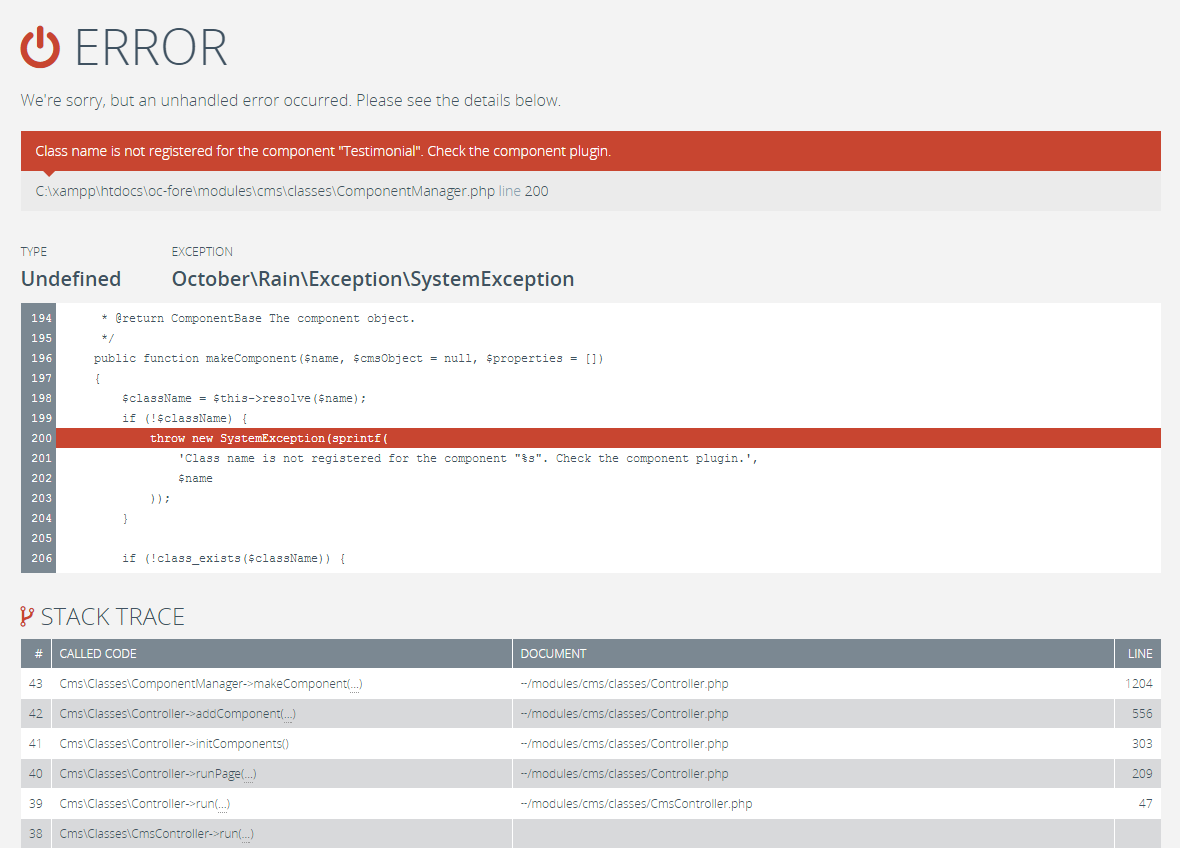
\includegraphics[width=\textwidth]{img/oc-exeption.png}
  \caption{De foutboodschap van OctoberCMS bevat voldoende informatie om het probleem te lokaliseren en verdere stappen te ondernemen.}
  \label{fig:OctoberCMS exceptie.}
\end{figure}

\noindent
Via dit overzicht moet het duidelijk worden voor de ontwikkelaar waar en waarom deze fout werd gegooid. Verdere stappen kunnen nu ondernomen worden om de fout op te lossen of de code te debuggen. 

\subsubsection{Versiebeheersysteem}
OctoberCMS laat zich heel eenvoudig beheren door een versiebeheersysteem. Doordat het systeem bestandsgebaseerd is geeft dit geen conflicten met betrekking tot de database. Front-end en back-end ontwikkelaars kunnen tegelijkertijd werken aan éénzelfde project zonder probleem. Eventuele conflicten waarbij elkaars code overschreven werd kan via een goede IDE (Integrated Development Environment) of editor worden samengevoegd en aangepast.

\subsection{Besluit}
Doordat bij Drupal alle acties in de back-end van de browser gebeuren, wordt dit ervaren als overrompelend. Een teveel aan verschillende opties en items maakt het menu overdreven groot en vergt ervaring alle knoppen en opties te leren kennen. De toevoeging van modules zorgt voor een uitbreiding van het menu, als ook opties binnen andere menu-items. OctoberCMS houdt de back-end in de browser overzichtelijk en implementeert enkel de nodige functies. Alle andere functionaliteiten worden in code aangepast.
\newline\newline
OctoberCMS is een flexibel systeem die zowel grote als kleinere projecten voor zijn rekening kan nemen. Bij een installatie 'from Scratch' is enkel de minimum functionaliteit en code aanwezig om het systeem te laten draaien. Geen gedoe met overschrijven van huidige code zoals het geval bij Drupal.
\newline\newline
Foutboodschappen worden in OctoberCMS gedetailleerd en gestructureerd opgebouwd als aparte pagina, waarmee je verder aan de slag kan. Drupal toont enkel een korte foutboodschap bovenaan de pagina die weinigzeggend is.
\newline\newline
Er kan besloten worden dat OctoberCMS op gebied van beheersbaarheid een stuk beter scoort dan Drupal 7.


\section{Database}
Bijna iedere applicatie komt in contact met een database, al is het nu om gewoon data op te halen of weg te schrijven. Een CMS maakt sowieso gebruik van een database. Verschillende elementen moeten in rekening gebracht worden bij het kiezen van een systeem en eventuele selectie van het soort database. Efficiëntie van een database kan een heikel punt vormen. De hoeveelheid query's die verstuurd worden en hoe lang deze query's er over doen. Of er al dan niet gebruik wordt gemaakt van caching, enz. Allemaal items om rekening mee te houden bij het evalueren van een systeem.

\subsection{Drupal}
Een installatie van Drupal 7 wordt meegeleverd met een verzameling van maar liefst 73 tabellen die een bestandsgrootte van 4.5MB innemen, waarvan 10 tabellen zullen dienst doen voor caching. Deze tabellen slaan alle wederkerende informatie op, zodat niet alle data telkens opnieuw volledig opgehaald moet worden. Op deze manier behaalt Drupal zijn gewenste performantie. 11 van de 73 tabellen hebben geen relatie met andere tabellen en bestaan dus op zichzelf. Overige tabellen kunnen opgedeeld worden in verschillende categorieën. 

\begin{itemize}
	\item{Field gerelateerde tabellen}
    \item{User gerelateerde tabellen}
    \item{Node gerelateerde tabellen}
    \item{Tussentabellen die User en Node tabellen linken}
\end{itemize}

\noindent
Deze tabellen zijn gekoppeld met elkaar via vreemde sleutel relaties.

\begin{figure}[!ht]
  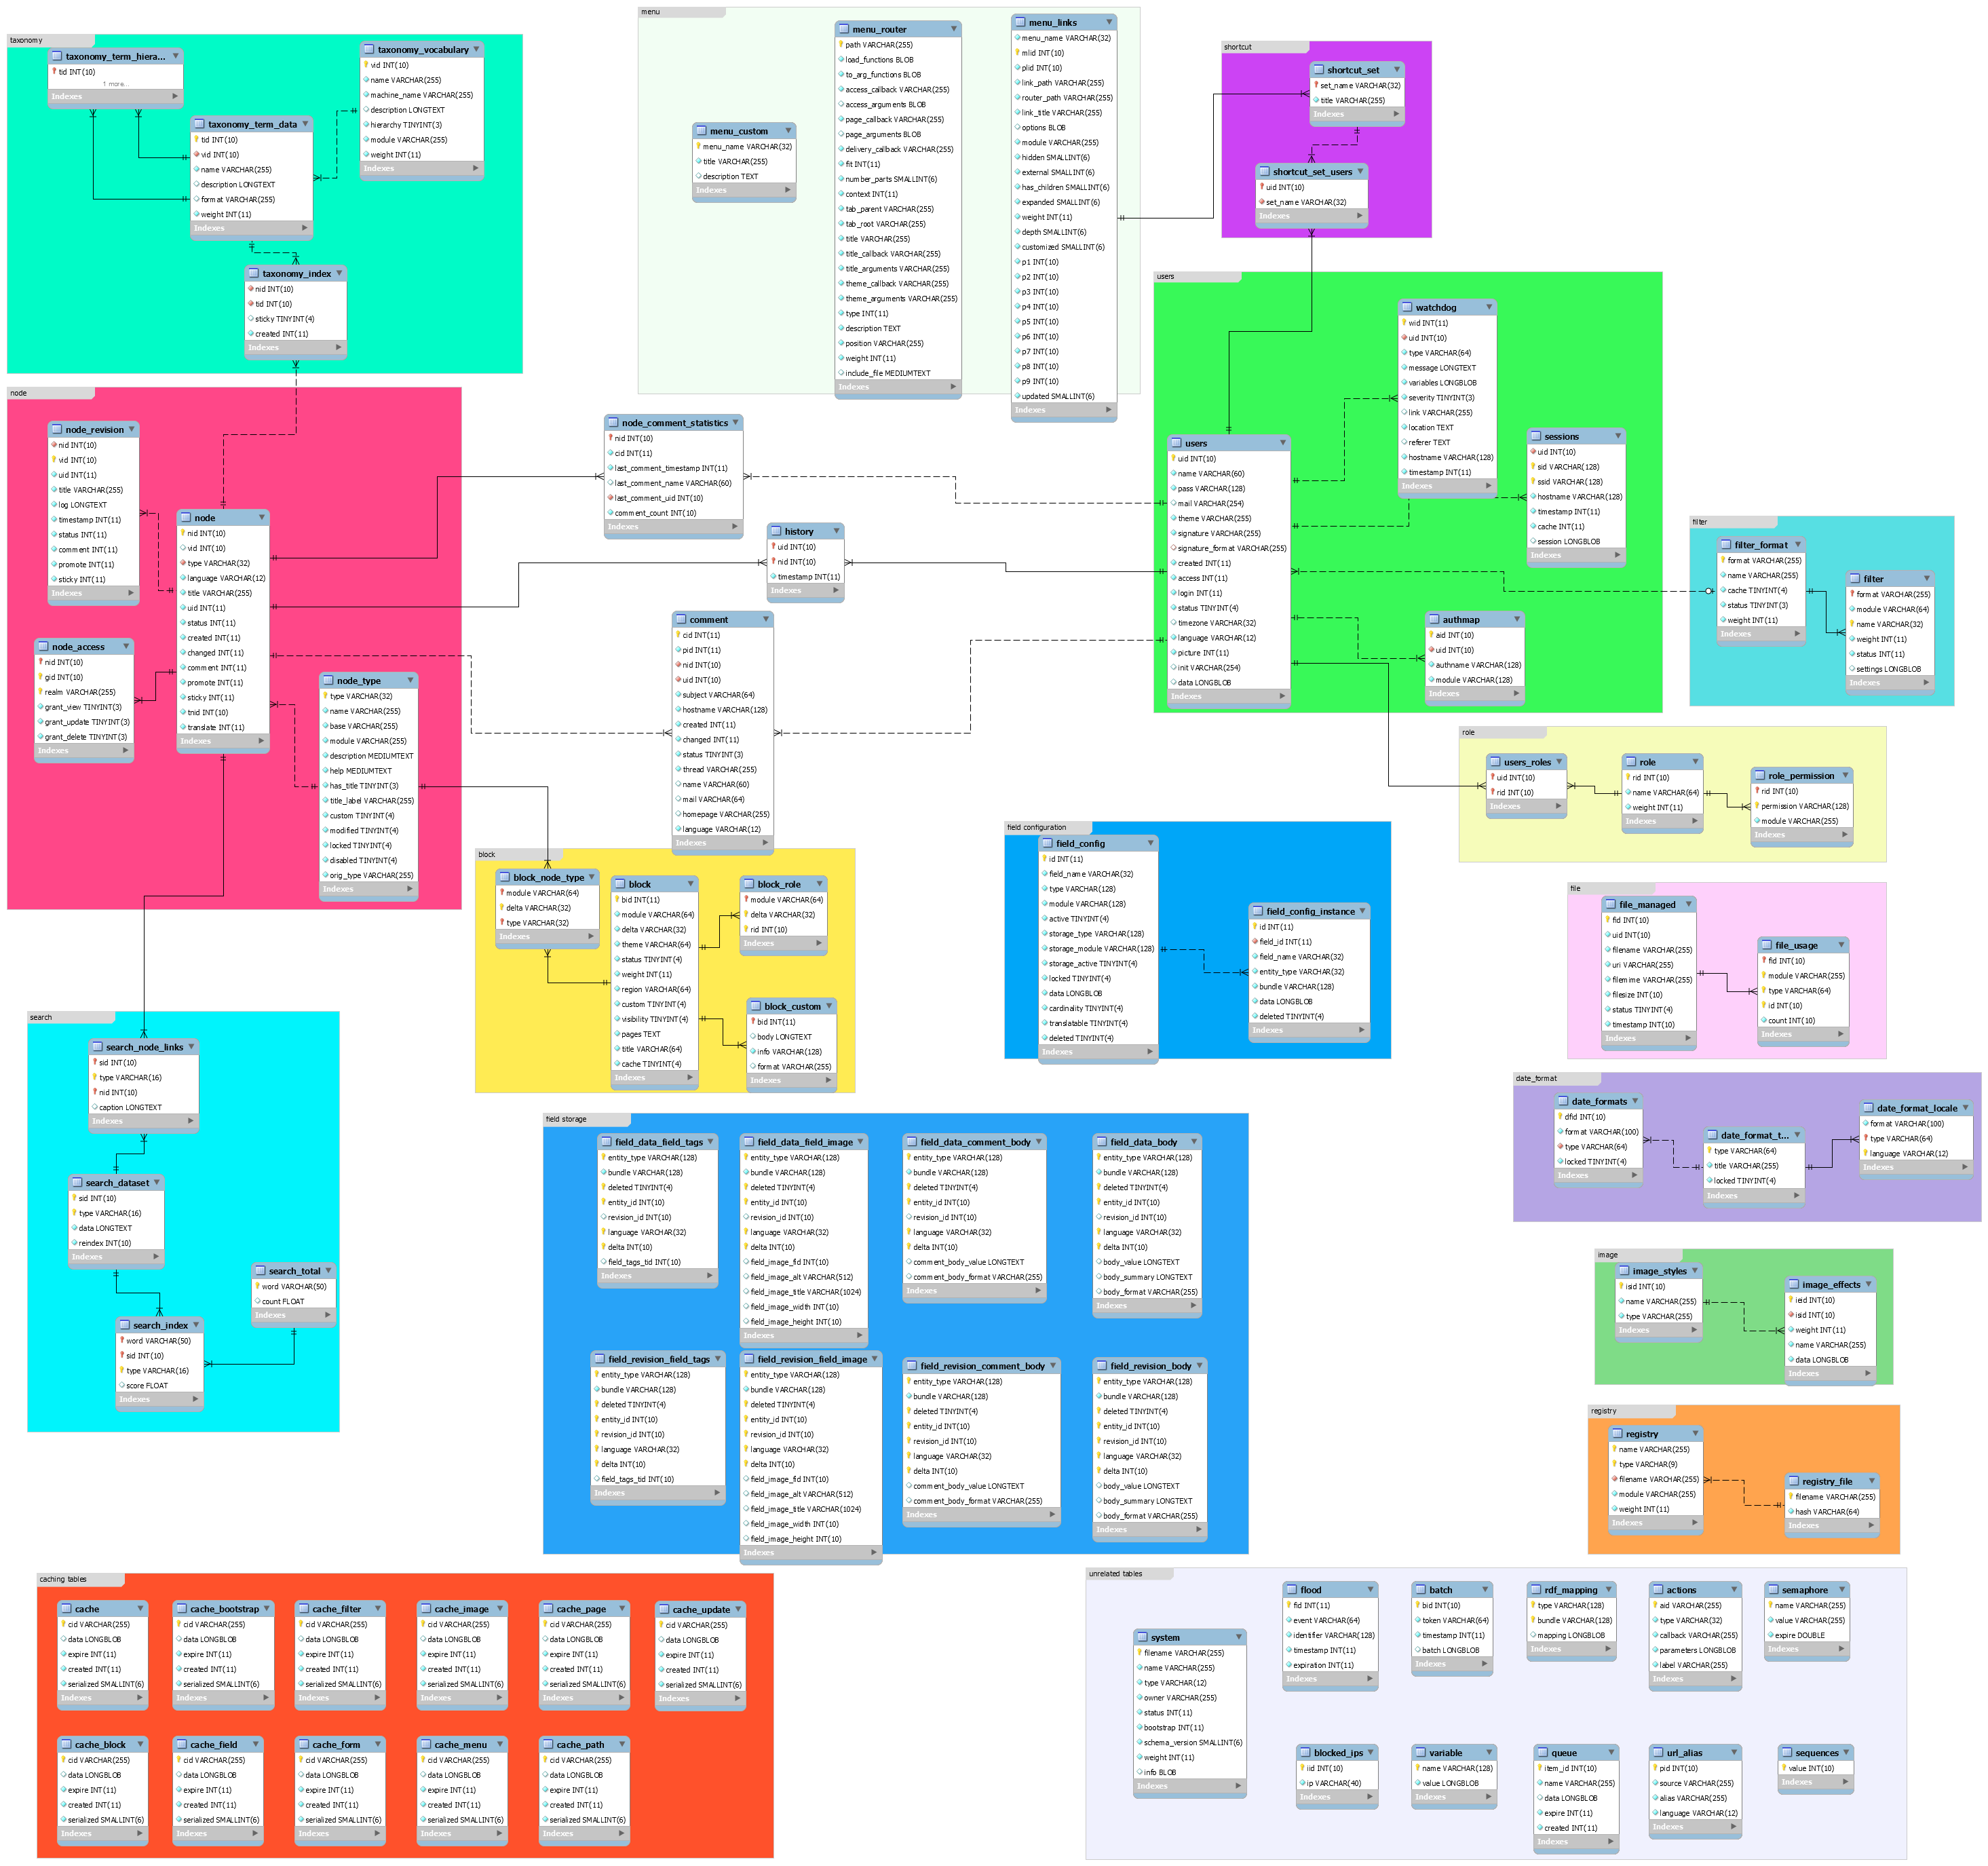
\includegraphics[width=\textwidth]{img/dr-database-erd.png}
  \caption{Bij de installatie van Drupal worden 73 tabellen aangemaakt.}
  \label{fig:Drupal core ERD.}
\end{figure}

\noindent
De hoeveelheid tabellen die enkel en alleen dienen om het systeem op te starten en te laten werken, is eerder aan de hoge kant. Drupal is modulair en zal voor het opbouwen van een site tientallen modules toevoegen. Aangezien deze modules communiceren met de database zal voor iedere module minimum één tabel worden aangemaakt. Deze nieuwe tabellen kunnen op hun beurt relaties bevatten met andere tabellen. Het gevolg van deze acties leidt tot een groter, ingewikkelder ERD (Entity-Relationship diagram). Een schema met alle entiteiten en relaties tussen deze entiteiten. Probeer daarom aandacht te vestigingen op de hoeveelheid modules en de combinatie ervan die je installeert. Zet alle onnodige modules uit om de belasting op de database zo laag mogelijk te houden.
\newline\newline
Qua flexibiliteit en hergebruik van data is Drupal verre van ideaal. De databasestructuur van Drupal is te ver genormaliseerd en bevat onnodige tabellen waardoor de volledige database niet de gewenste flexibiliteit bevat. Wanneer we de database van Drupal op een andere manier willen hergebruiken zien we dat dit zo goed als onmogelijk blijkt te zijn.

\subsection{OctoberCMS}
Een nieuwe installatie van OctoberCMS maakt 23 tabellen aan die een bestandsgrootte innemen van 495KB. Bij het creëren van nieuwe plugins kunnen extra tabellen worden toegevoegd. Het aantal toegevoegde tabellen is afhankelijk van de complexiteit van de plugin. De toename van tabellen blijft beheerst net zoals de relaties tussen tabellen. Deze tabellen en hun onderlinge relaties worden in code aangemaakt. Tabellen die aangemaakt worden bij installatie kunnen grotendeels opgesplitst worden in categorieën.

\begin{itemize}
	\item{Systeem gerelateerde tabellen}
    \item{User gerelateerde tabellen}
\end{itemize}

\noindent
De overige tabellen zijn op zichzelf staande tabellen en kunnen niet gecategoriseerd worden. Over het algemeen zien we dat de structuur van het ERD eenvoudig is opgebouwd. Er is slechts één tussentabel waarbij een relatie loopt. Dit is de tabel 'backend\_users\_groups'. Er is geen sprake van ingewikkelde relaties met vreemde sleutels.
\newline\newline
Zoals reeds aangehaald kunnen er bij het creëren van plugins één of meerdere tabellen worden aangemaakt. Deze tabellen worden allemaal voorafgegaan door de unieke naam van de ontwikkelaar gevolgd door de naam van de plugin en de tabelnaam. 


\begin{figure}[!ht]
  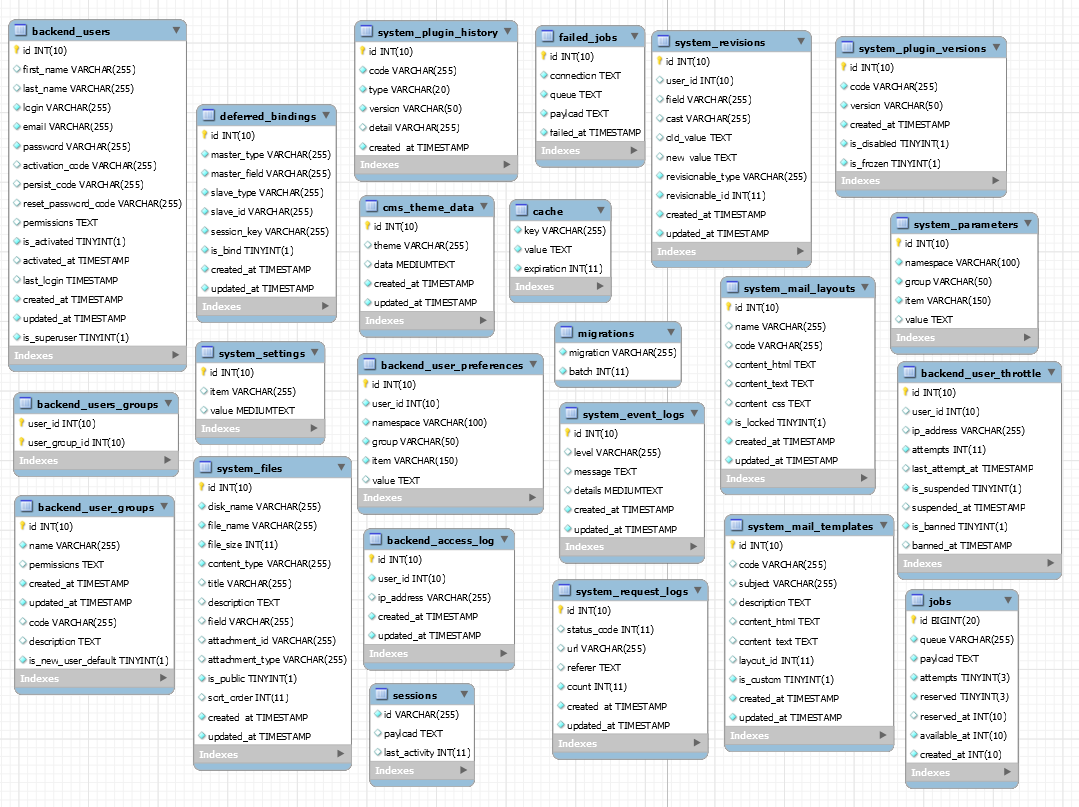
\includegraphics[width=\textwidth]{img/oc-database-erd.png}
  \caption{Bij de installatie van OctoberCMS worden 23 tabellen aangemaakt.}
  \label{fig:OctoberCMS core ERD.}
\end{figure}

\noindent
OctoberCMS voorziet één tabel voor caching. Hoewel de meeste cache gerelateerde acties worden voorzien door OctoberCMS zelf, is het mogelijk ook manueel functies aan te maken om eigen data te cachen.

\begin{minted}{c}
	Cache::put('key', 'value', $minutes);
    $value = Cache::get('key');  
\end{minted}

\noindent
Via deze eenvoudige methoden kan je via de 'put' functie elementen voor een bepaalde tijd (\$minutes) opslaan in de cache en vervolgens terug ophalen via de 'get' methode.
\newline\newline
De databasestructuur van OctoberCMS is flexibel. De database kan op eenvoudige wijze gebruikt worden door andere applicaties. Het doorzoeken van tabellen levert een snel, duidelijk en volledig resultaat op.

\pagebreak

\subsection{Besluit}
De bestandsgrootte en het aantal tabellen bij installatie van de database van Drupal is groot. Met een enkel toenemende database door modules, is het belangrijk de controle van modules in het oog te houden. OctoberCMS start met een select aantal tabellen om het systeem te laten werken. Geen overbodige tabellen waarvan het systeem misschien nooit gebruik maakt. 
\newline\newline
De database van Drupal is te ver genormaliseerd waardoor de duidelijke structuur en flexibiliteit niet ideaal is. Het hergebruiken of extraheren van gegevens uit de database is onbegonnen werk. Dit in tegenstelling tot OctoberCMS. Als ontwikkelaar is het interessanter werken met een database zoals deze aangeleverd wordt bij OctoberCMS.